\section{Labeling Instructions \& Quality}
\label{appendix:label_instruct}


\begin{figure*}
\centering
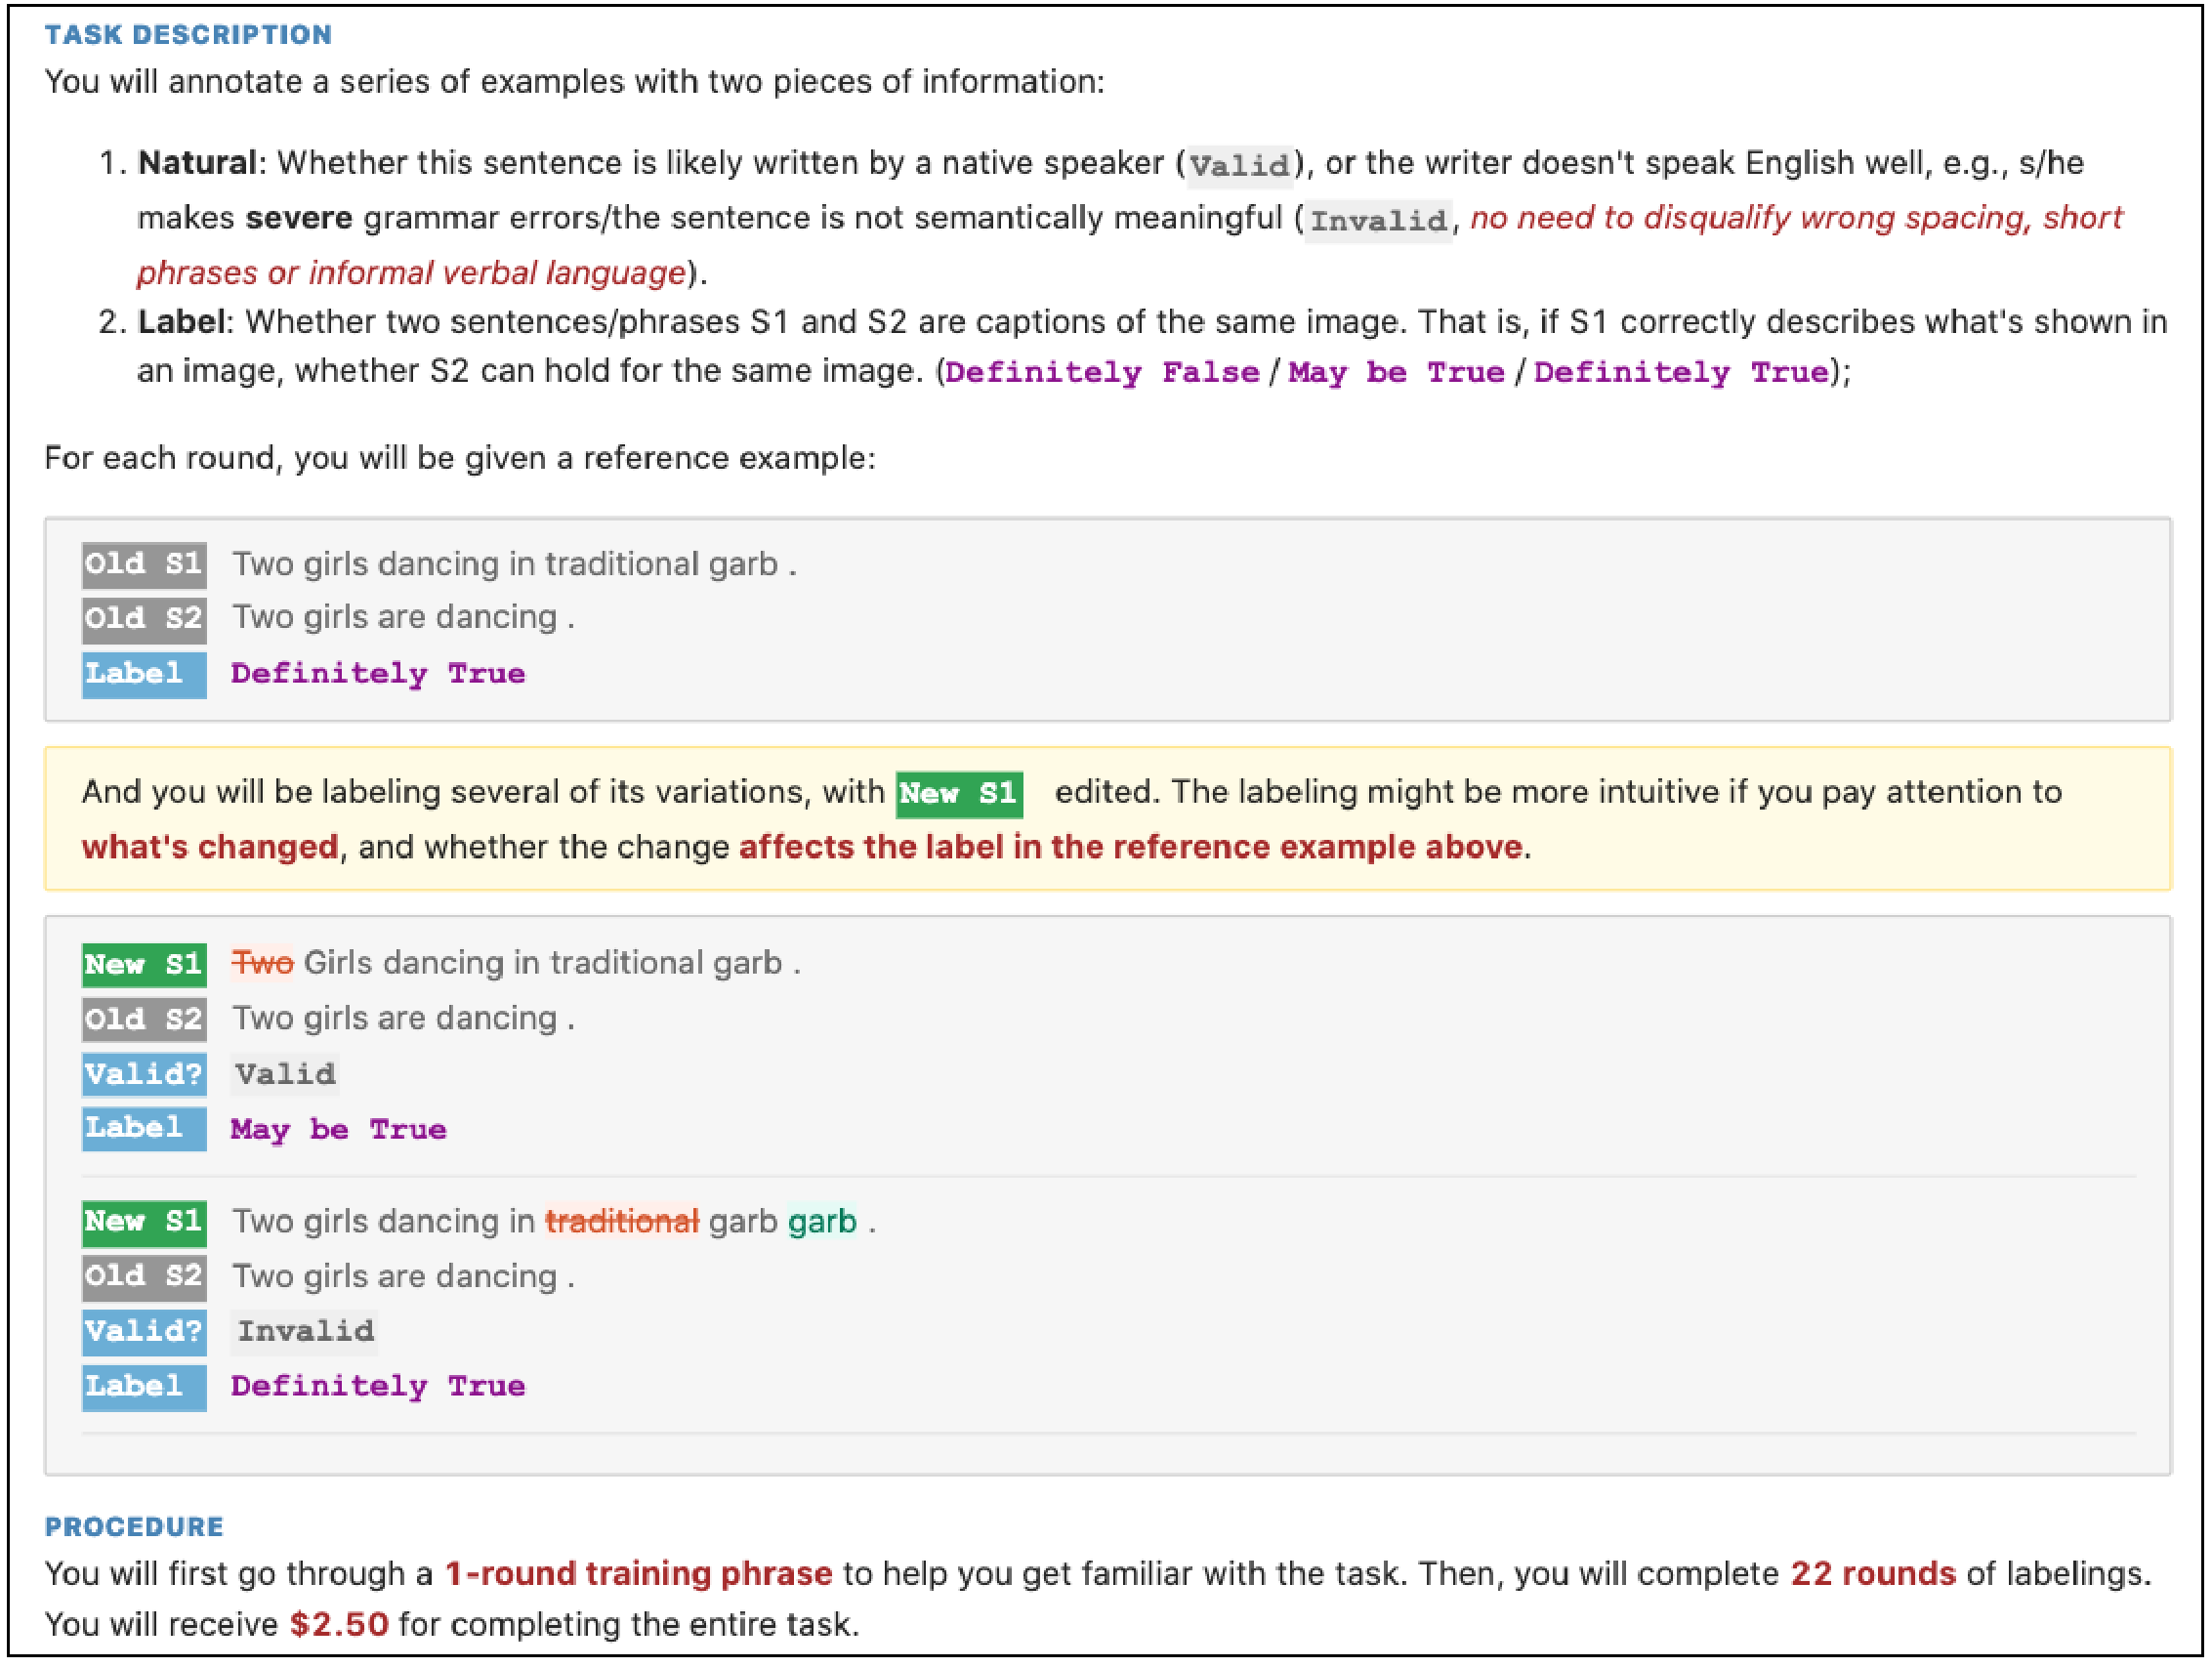
\includegraphics[width=1\textwidth]{figures/mturk_instruction.pdf}
\vspace{-15pt}
\caption{A sample instruction for the \nli task, with annotators providing labels based for the perturbed hypotheses (\emph{New S2}). Instructions are similar for \qqp and \sst, except for the label definitions and the examples. \wts{Change to hypothesis screenshot.}}
\vspace{-10pt}
\label{fig:mturk_instruction_detail}
\end{figure*}

\paragraph{Procedure\footnote{A complete annotation demo is available at \mturkurl.}}
The study started with an introduction, in which we explained the context and tasks (Figure~\ref{fig:mturk_instruction_detail}): 
``given a reference example, the crowdworker should annotate its perturbed variations, based on whether the perturbation is valid (\emph{sounds natural}), and the classification task label.''
To familiarize them with the task, we asked them to complete 1-2 training rounds, and explained the expected labels.
The annotator then completed 22 tasks, each labeling 3 variations of a single example.
The 22 rounds consisted of 20 actual labeling tasks and 2 extra ``gold rounds'' (6 labeled examples), with unambiguous examples and known groundtruth labels, which later served as filters for high quality crowdworkers.
As a result, each annotator contributed $20 \times 3=60$ labels.
The median task completion time was around 15-20 minutes (14.9 for \qqp, 16.7 for \sst, and 19.8 for \nli), and participants received an average payment of \$2.5 (equivalent to an hourly wage of \$7.5).

\paragraph{Participants}
We recruited participants from Amazon's Mechanical Turk (MTurk), limiting the pool to subjects from within the United States with a prior task approval rating of at least 97\% and a minimum of 1,000 approved tasks.

\paragraph{Data quality}
We applied two filtering strategies: 
(1) \emph{High quality worker.} 
We only kept data from participants whose median labeling time was more than 18 seconds and correctly labeled at least 4 gold examples (out of 6), or who correctly labeled all gold ones.
(2) \emph{Majority vote labeling.}
We collected two annotations per perturbation, and only kept data points that at least one annotator deems \emph{valid}, and both annotators agree on a particular \emph{class label.}

As such, when set out to collect augmentations on 1,000 original examples (thus 3,000 perturbations), we typically collect perturbations for 1,000 perturbations on 600 original examples.
One of the authors labeled a subset of 100 perturbations on 100 original examples in \sst, and reached high agreement with the majority-voted results ($\kappa=0.77$, the raw labeling agreement $88\%$).
